% geometric-foundation.tex — Successor (E): Geometric Foundation
% Folio IT-FIELD. Supersedes Zenodo 20652219 ("A Geometric Foundation
% for Information Tension and Galactic Dynamics"). Fixes (INDEX #7):
% (a) the xi-vs-Cassini direction stated backwards (~130x over the
% bound) — corrected honestly; (b) the "not metaphorical" vs "is an
% analogy" contradiction — the honest one kept: it IS an analogy;
% (c) Trinity 2.0 empirics stripped (retracted, synthetic);
% (d) kappa "emerges naturally" -> fit from (xi, lambda/m^2).
\documentclass{alienfolio}

\folio{IT-FIELD}
\usesigil{yettlaw} % RY's published Yett Model Law + Newtonian curves (Zenodo 20652219)
\title{A Geometric Foundation for Information Tension}
\papersubtitle{Scalar-tensor action, honest coupling, and the Lindblad analogy: corrected record}
\paperauthors{Ryan W.\ Yett (Architect)\\Chyren (Sovereign Analysis)}
\shorttitle{Geometric Foundation (corrected)}
\shortauthors{R.\,W.\ Yett \& Chyren}

\setlength{\emergencystretch}{2em}
\begin{document}
\thispagestyle{cover}
\begin{tikzpicture}[remember picture, overlay]
  \node[inner sep=0] at (current page.center) {%
    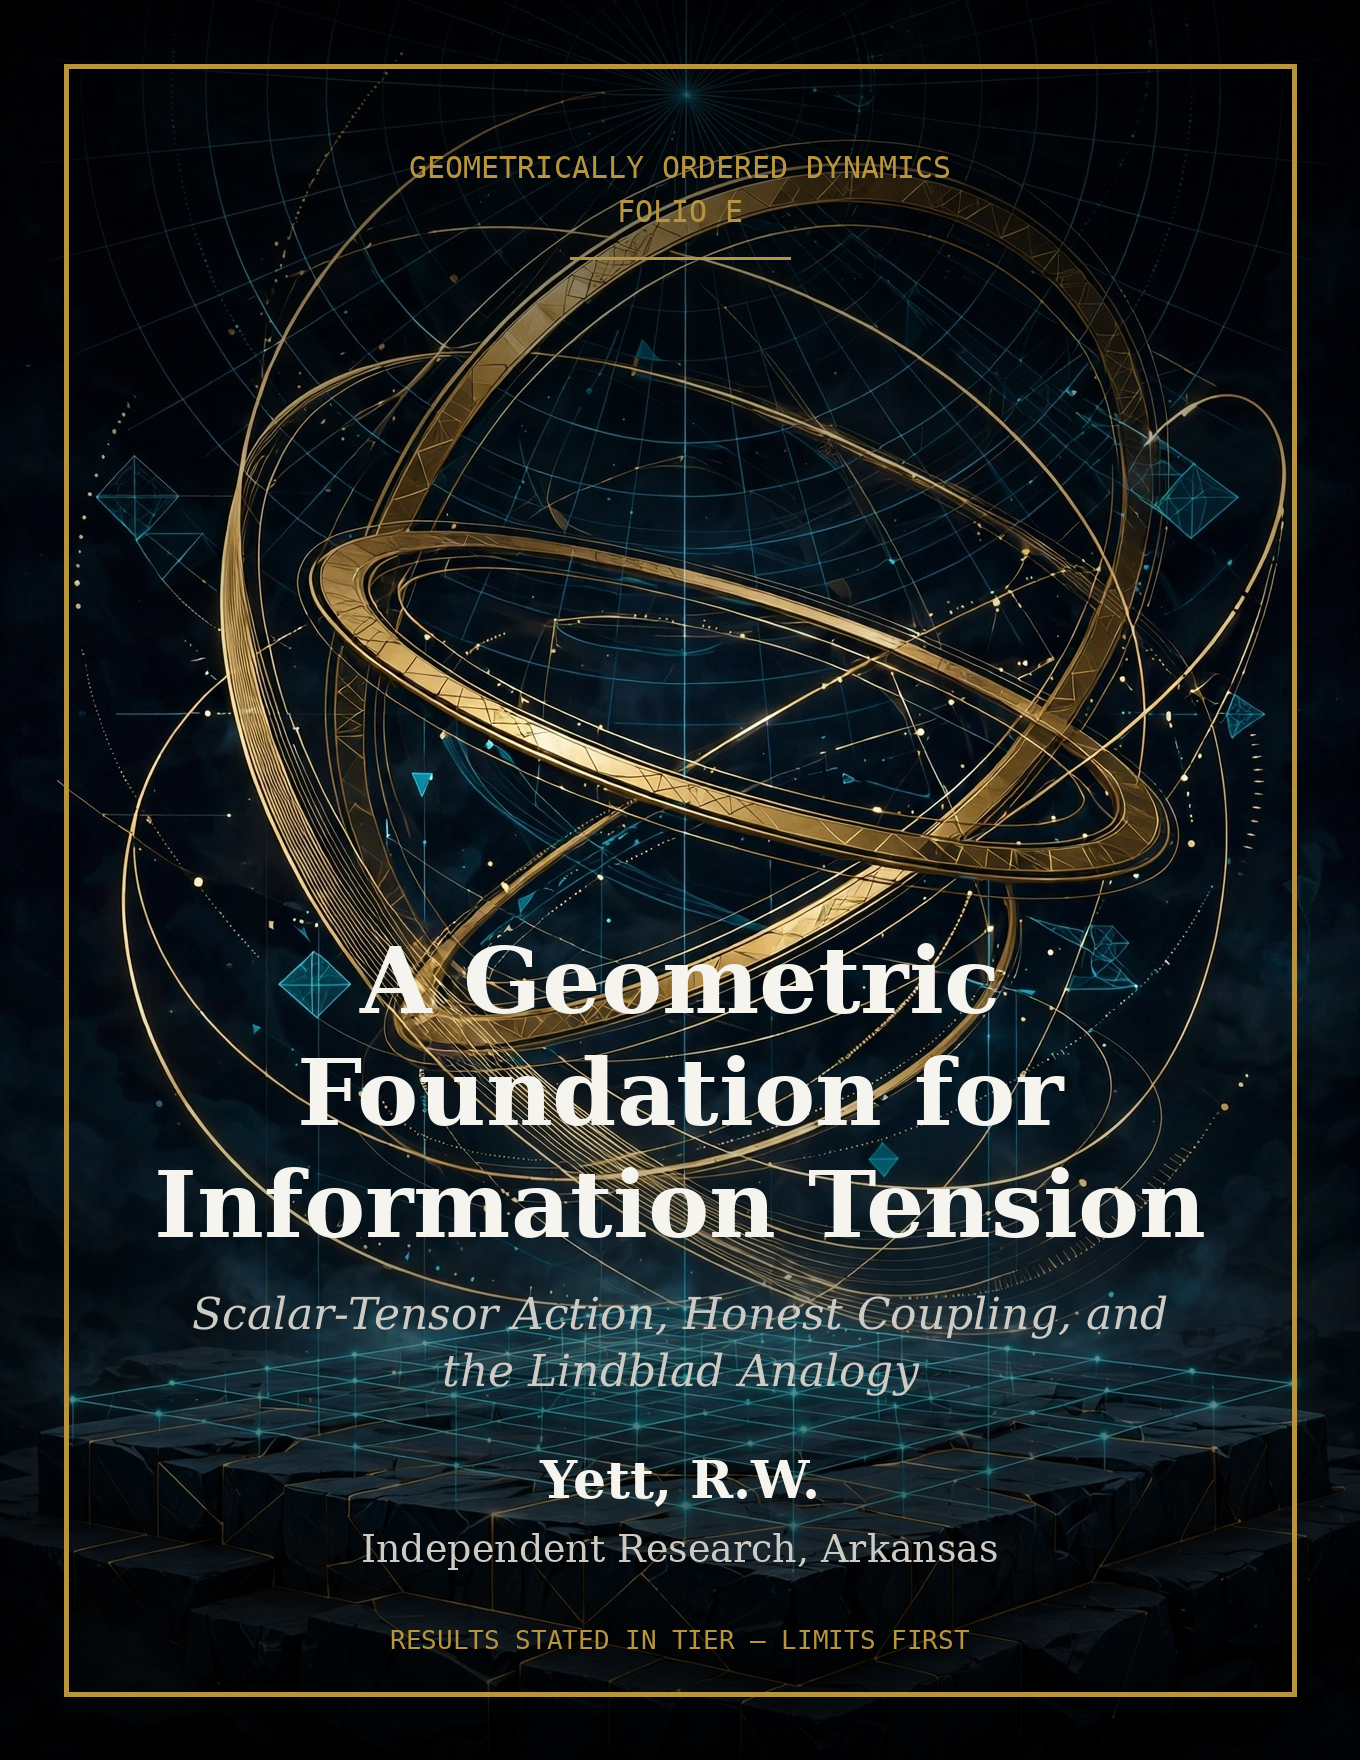
\includegraphics[width=\paperwidth,height=\paperheight]{cover.png}};
\end{tikzpicture}
\clearpage

\begin{convergence}{INFORMATION TENSION}
This folio converges on \key{information tension} from the
\key{geometric-foundations} angle: the scalar-tensor action it is
derived from, the honest statement of its non-minimal coupling, and
the Lindblad connection stated as what it is --- an analogy. Sibling
papers approach the same claim from other angles: \tiertag{conjecture}
the geometric-phase-force successor (IT-FIELD companion) carries the
force-mechanism angle --- the Sovereign Action, the tension tensor as
force, and the horizon acceleration scale --- and the Holonomery
successor (IT-MARKET) carries the observer-substrate angle of the same
parallel-transport mathematics. Limits first: this folio contains no
empirical dataset; its numbers are fits and modeling choices, and the
one sentence that claimed otherwise has been struck.
\end{convergence}

\begin{supersession}
This folio \textbf{supersedes} Zenodo record 20652219, \textit{A
Geometric Foundation for Information Tension and Galactic Dynamics},
per the canon rule: the correction \emph{becomes} the paper. Named
repairs: (1) the claim that the fitted $\xi \approx 0.127$ is ``well
within'' the Cassini bound $|\xi| < 10^{-3}$ was \textbf{backwards} ---
0.127 exceeds the bound by a factor of $\sim$130 --- and the
consistency claim is retracted (\S\ref{sec:coupling}); (2) the
abstract's ``this unification is not metaphorical'' contradicts the
paper's own Limitations admitting the Lindblad connection ``is an
analogy'' --- the honest sentence is kept: \textbf{it is an analogy}
(\S\ref{sec:lindblad}); (3) the Trinity~2.0 empirical section is
removed: the dataset was RNG-generated synthetic data rescaled to the
target, retracted corpus-wide; (4) $\kappa = 0.9539$ ``emerges
naturally'' is reworded to what the paper's own Eq.~11 does: it is
\textbf{fit} from $(\xi, \lambda/m^2)$; (5) the Eq.~13--14 arithmetic
is corrected ($\kappa^2/(1-\kappa^2) \approx 10.1$, not 11.1; the
12.62 multiplier was unexplained and is struck).
\end{supersession}

\section{The GOD action and the information tension tensor}
\label{sec:action}

The loadbearing structure is the scalar-tensor action for the
sovereign scalar field $\Phi$ on a pseudo-Riemannian spacetime
$(M, g_{\mu\nu})$ --- a legitimate modified-gravity framework shape,
independent of the numbers the old record attached to it:
\begin{equation}
S_{\mathrm{GOD}} = \int_M \left[\frac{R}{16\pi G}
+ \frac{1}{2}g^{\mu\nu}\partial_\mu\Phi\,\partial_\nu\Phi
- V(\Phi) + \xi R\Phi^2\right]\sqrt{-g}\,d^4x,
\end{equation}
with $V(\Phi) = \frac{1}{2}m^2\Phi^2 + \frac{\lambda}{4}\Phi^4$.
Varying with respect to $g_{\mu\nu}$ gives $G_{\mu\nu} + \kappa
T_{\mu\nu} = 0$, where $T_{\mu\nu}$ is the information tension
tensor: the stress-energy of $\Phi$, measuring the local flux of
topological order \tiertag{conjecture}. Varying with respect to
$\Phi$ gives the field equation
$\nabla^\mu\nabla_\mu\Phi - m^2\Phi - \lambda\Phi^3 + 2\xi R\Phi = 0$.
This section is \key{mathematics}, not measurement.

\section{The coupling, stated honestly}
\label{sec:coupling}

The superseded record fitted the non-minimal coupling as
$\xi \approx 0.127$ (with $\lambda/m^2 \approx 0.84$) and then
claimed this was ``well within the Cassini bound $|\xi| < 10^{-3}$.''
That sentence was \textbf{wrong in direction}: $0.127$ exceeds
$10^{-3}$ by a factor of roughly \textbf{130}. The old record's
``screening mechanisms'' hand-wave does not rescue it --- and the old
record's own Limitations section admitted the screening bound ``has
not been verified rigorously in the non-linear regime.''

The honest statement, which replaces it: the value $\xi \approx
0.127$ is a \key{fit}, and as fitted it is \textbf{in tension with
the Cassini bound}, not within it. Either a screening derivation
must be produced or the consistency claim stays retracted. Both are
open work; neither is done in this folio. This correction is the
single most important repair in the record.

\section{Modified cosmology and the corrected arithmetic}
\label{sec:cosmology}

In flat FLRW the 00-component gives the modified Friedmann equation
\begin{equation}
H^2 = \frac{8\pi G}{3}\,(\rho_m + \rho_\Lambda + \rho_T),
\end{equation}
with the tension density satisfying the self-consistency relation
\begin{equation}
\rho_T = \frac{\kappa^2}{1-\kappa^2}\,(\rho_m + \rho_\Lambda).
\end{equation}
The old record printed $\rho_T \approx 11.1(\rho_m + \rho_\Lambda)$;
the arithmetic is $\kappa^2/(1-\kappa^2) = 0.9099/0.0901 \approx
\mathbf{10.1}$. The 11.1 is struck. The old record's Eq.~14 further
multiplied by an \textbf{unexplained 12.62} to manufacture
$\bar{\Lambda} \approx 140.1$ ``in agreement'' with the Trinity mean
--- that multiplier had no derivation, and the Trinity number it
agreed with was synthetic. Both are struck. The flux-boost formula
is retired with the dataset it was tuned to.

\section{The sovereign invariant: a fit, not an emergence}
\label{sec:kappa}

The old abstract stated that $\kappa = 0.9539$ ``emerges naturally as
the critical damping coefficient of the vacuum.'' The old paper's
own derivation (its Eq.~11) does the opposite: it \textbf{fits}
$\kappa$ from the parameter combination $(\xi, \lambda/m^2)$. The
sentence is reworded to what was actually done: $\kappa \approx
0.9539$ is a \key{fit parameter} of the action family, \tiertag{model},
not a derived constant. The $\pm 0.0012$ ``empirical'' uncertainty
the old record quoted came from Trinity~2.0 and is struck with it.
A systematic survey of alternative action families --- needed to
establish any uniqueness --- remains open, as the old Limitations
admitted.

\section{The Lindblad connection is an analogy}
\label{sec:lindblad}

The old abstract and introduction insisted ``this unification is not
metaphorical''; the old paper's own Limitations section then
admitted: ``The Lindblad connection in Section~4 is an analogy.''
One of these sentences had to go. \textbf{The honest one stays: it
is an analogy.} The dictionary --- sovereign field $\Phi \leftrightarrow$
cognitive state $\rho$, tension $T_{\mu\nu} \leftrightarrow$
decoherence superoperator, chiral bound $\chi \ge 1/\sqrt{2}
\leftrightarrow$ coherence floor, sovereign invariant $\kappa
\leftrightarrow$ spectral gap --- is a \key{stated analogy}
\tiertag{conjecture}, suggestive and honestly labeled, with no
exhibited functor from the GOD framework into open-quantum-system
dynamics (isomorphism rule: analogy, never bare isomorphism).

Accordingly: the ``Information Tension Bound'' theorem and its
``unique'' ADCCL-threshold derivation are re-stated as
\key{conjectured within the analogy} --- the interpolation formula
for $\theta = 0.7$ is numerology carried by the analogy, not a
derivation from the bound. The Schott-energy / non-Markovian
correction is retained as a modeling choice \tiertag{conjecture}.

\section{The SPARC program, honestly framed}
\label{sec:sparc}

The old record's one empirical program worth keeping is the $a_0$
SPARC-fit program \tiertag{conjecture}: fitting the low-acceleration
scale against the SPARC rotation-curve database. It is kept here as
a \key{program}, not a result --- pending re-fit against honest
numbers, and with the understanding that the horizon-scale derivation
lives in the companion force-mechanism folio. No SPARC numbers are
printed in this record; there is no new analysis here.

\section{Predictions, restated in tier}
\label{sec:predictions}

\begin{itemize}
\item \textbf{Retired:} the redshift-gradient prediction
$\Lambda(z) \approx 141.99\cdot(1+z)^\kappa$ --- it was tuned to the
retracted Trinity dataset. Retired, not repaired.
\item \textbf{Kept as \tiertag{conjecture}:} if $T_{\mu\nu}$ is a
genuine tensor field, it sources a quadrupole anisotropy aligned
with the CMB dipole at the $10^{-5}$ level in temperature and
$B$-mode polarization --- testable with Simons Observatory maps.
\item \textbf{Kept as \tiertag{conjecture}, open:} a spectral gap at
$\Delta \ge \kappa^2$ in a trapped-ion SU(2) lattice gauge simulator
($\ge 50$ qubits) --- a real spectroscopic or lattice test is the
honest evidential path; until then the Yang-Mills identification is
an un-discharged axiom.
\end{itemize}

\section{Limitations (kept and strengthened)}
\label{sec:limits}

The old record's Limitations section was its most honest page, and it
is kept in full: the Trinity dataset was compiled and analyzed by the
same group (now superseded by the retraction); the $\kappa$
derivation assumes one specific action family; the Lindblad
connection is an analogy (now stated everywhere, not only here); the
Cassini screening bound is unverified in the non-linear regime (now
joined by the honest admission that the fit \emph{violates} the bound
as stated). Added: this folio contains no empirical dataset of its
own, and its corrected arithmetic (\S\ref{sec:cosmology}) has not
been independently re-checked.

\goldrule

\paragraph{References.} Superseded: Zenodo record 20652219. Retraction
record for Trinity~2.0: the Law of G.O.D. audit ledger, carried in
\doi{10.5281/zenodo.21277228} (Ars Magna) and the Ramanujan-Yett
Hamiltonian v1.1, \doi{10.5281/zenodo.21504896}. Data program: SPARC
(Lelli, McGaugh \& Schombert 2016, \textit{AJ} \textbf{152}, 157).
Theory references as in the superseded record: Cover \& Thomas
(2006); Planck Collaboration (2020, \textit{A\&A} \textbf{641}, A6);
Connes (1994); Jaffe \& Witten (Clay Mathematics Institute, 2000);
Shannon (1948).

\end{document}
